\documentclass[10pt]{article}
\usepackage[a4paper, margin=2cm]{geometry}
%\usepackage{fullpage}
\usepackage[T1]{fontenc}
\usepackage[utf8]{inputenc}
\usepackage{graphicx}
\usepackage{mathpazo}
\pagenumbering{arabic}
\usepackage{siunitx}
\usepackage{amsmath}
\usepackage{mathtools} % Para poder usar "\Aboxed"
\usepackage{cancel} % Para usar "\cancel", de https://tex.stackexchange.com/questions/537955/how-do-cross-out-text-in-math-mode
\usepackage{multicol}
\usepackage[spanish]{babel}
\usepackage{steinmetz}
\DeclareSIUnit\voltampere{VA}
\DeclareSIUnit\var{VAr}
\setlength\parindent{0pt} % no indent

% Numbering pages on the right footer:
% (https://tex.stackexchange.com/questions/153167/how-to-set-page-number-at-right-footer)
\usepackage{fancyhdr}
% Turn on the style
\pagestyle{fancy}
\fancyhf{} % sets both header and footer to nothing
\renewcommand{\headrulewidth}{0pt} % To remove the top horizontal line created by default by "fancyhdr", from here: https://tex.stackexchange.com/questions/13896/how-to-remove-the-top-horizontal-bar-in-fancyhdr
% Set the right side of the footer to be the page number
\fancyfoot[R]{\thepage}


\usepackage{minibox} % Para poder partir el texto en 2 líneas usando "underbrace" u "overbrace", info aquí: https://tex.stackexchange.com/questions/8680/how-can-i-insert-a-newline-in-a-framebox


\usepackage{xparse} % For "overbrace/underbrace but with an arrow instead", from https://tex.stackexchange.com/questions/8720/overbrace-underbrace-but-with-an-arrow-instead

% Para poner flechas sobre los signos de igual, de aquí: https://tex.stackexchange.com/questions/8720/overbrace-underbrace-but-with-an-arrow-instead
\NewDocumentCommand{\overarrow}{O{=} O{\uparrow} m}{%
  \overset{\makebox[0pt]{\begin{tabular}{@{}c@{}}#3\\[0pt]\ensuremath{#2}\end{tabular}}}{#1}
}
\NewDocumentCommand{\underarrow}{O{=} O{\downarrow} m}{%
  \underset{\makebox[0pt]{\begin{tabular}{@{}c@{}}\ensuremath{#2}\\[0pt]#3\end{tabular}}}{#1}
}



\begin{document}

\large{\textbf{Ejercicio 8 de la colección de problemas}}

\vspace{3mm}
\large{\textbf{Enunciado}}:

\vspace{5mm}

\begin{minipage}{0.65\linewidth}
    \vspace{-24mm}
    En el circuito de la figura, donde se sabe que la carga inicial de los condensadores era de $\qty{10}{\micro\coulomb}$ para $C_1$ y de $\qty{20}{\micro\coulomb}$ para $C_2$, con las polaridades indicadas, se pide determinar:
    
    \begin{enumerate}
        \item Intensidades de corriente señaladas
        \item Potenciales en los puntos A, B, C, D, E y F
    \end{enumerate}
\end{minipage}
\hfill
\begin{minipage}{0.25\linewidth}
    \textbf{Datos}:
    \vspace{2mm}
    
    $R_1 = R_2 = R_3 = \qty{10}{\ohm}$\\
    $R_4 = R_5 = \qty{30}{\ohm}$\\
    $C_1 = \qty{10}{\micro\farad}$\\    
    $C_2 = \qty{20}{\micro\coulomb}$\\
    $q_{C_1,0} = \qty{10}{\micro\farad}$\\
    $q_{C_2,0} = \qty{20}{\micro\farad}$\\
    $L_1 = \qty{1}{\micro\henry}$\\
    $\epsilon_1=\qty{90}{\volt}$\\
    $\epsilon_2 = \qty{60}{\volt}$\\
    $\epsilon_3 = \qty{30}{\volt}$    
\end{minipage}

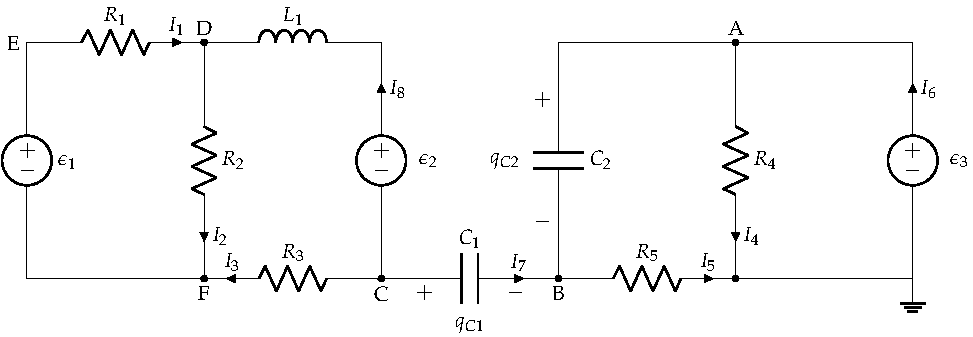
\includegraphics[scale=1.08]{figs/mallas_carga_inicial.pdf}

%\vspace{2mm}

\hrulefill

\vspace{5mm}
\textbf{Solución}:
\vspace{4mm}

Sustituimos los condensadores por circuitos abiertos, lo que implica que por las ramas correspondientes no puede circular corriente:

\vspace{-2mm}
\begin{align*}
  I_5 &= \qty{0}{\ampere}\\
  I_7 &= \qty{0}{\ampere}
\end{align*}

\vspace{-12mm}
\begin{center}
  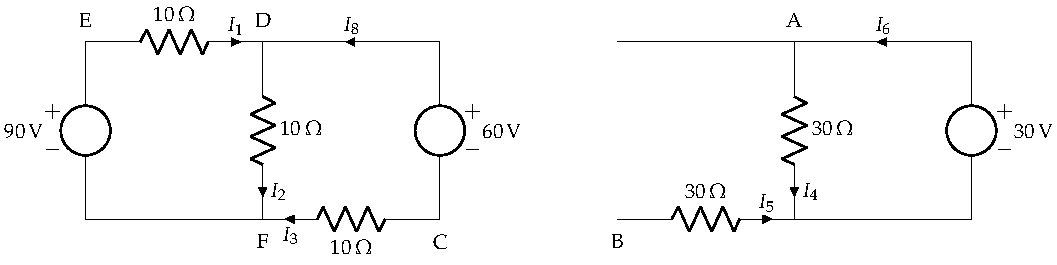
\includegraphics[scale=0.99]{figs/BT1_10_mod.pdf}
\end{center}

En consecuencia:

\vspace{-5mm}
\begin{align*}
  I_3 &= -I_8\\
  I_4 &= I_6
\end{align*}

\vspace{2mm}
Además, la bobina $L_1$ se sustituye por un cortocircuito.

Dado que el circuito original está ``partido'' en dos porciones inconexas, podemos analizar de manera independiente cada una de las dos porciones. Si aplicáramos la ecuación general de mallas al circuito en su conjunto, obtendríamos una matriz con ceros en los elementos comunes entre la malla 3 (malla en la que se incluye el generador 3), y las mallas 1 y 2, por lo que el sistema de ecuaciones $3\times 3$ sería separable en dos partes (de dimensiones $2\times 2$ y $1\times 1$).

\vspace{5mm}
Por lo tanto, en el circuito de la izquierda se tienen dos mallas, considerando las corrientes de malla mostradas en la siguiente figura:

\vspace{3mm}
\begin{minipage}{0.5\linewidth}
    \begin{center}
      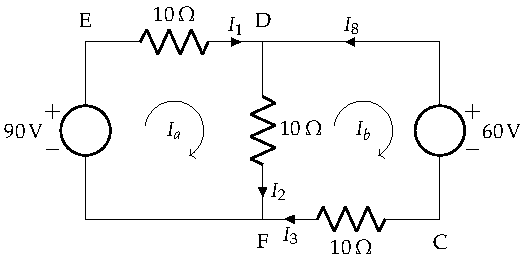
\includegraphics{figs/BT1_10_izq_mallas.pdf}
    \end{center}
\end{minipage}
\hfill
\begin{minipage}{0.4\linewidth}
    \begin{equation*}
      \begin{bmatrix}
        R_1 + R_2 & -R_2\\
        -R_2 & R_2 + R_3\\
      \end{bmatrix} \cdot %
      \begin{bmatrix}
        I_a\\
        I_b
      \end{bmatrix} = %
      \begin{bmatrix}
        \epsilon_A\\
        -\epsilon_B
      \end{bmatrix}
    \end{equation*} 
\end{minipage}






\vspace{4mm}
La solución de este sistema es:

\vspace{-5mm}
\begin{align*}
  I_a &= \qty{4}{\ampere}\\
  I_b &= \qty{-1}{\ampere}
\end{align*}

siendo:

\vspace{-5mm}
\begin{equation*}
  I_1 = I_a \, , \qquad\quad
  I_2 = I_a - I_b \, , \qquad\quad
  I_3 = I_b \, , \qquad\quad
  I_8 = -I_b
\end{equation*}

\vspace{2mm}
En el circuito de la derecha tenemos una única malla:

\begin{equation*}
  \epsilon_3 = I_4 \cdot R_4 \quad \rightarrow \quad I_4 = \qty{1}{\ampere}
\end{equation*}

\vspace{-2mm}
Por tanto:

\vspace{-3mm}
\begin{equation*}
  \boxed{I_1 = \qty{4}{\ampere}} \, , \; 
  \boxed{I_2 = \qty{5}{\ampere}} \, , \; 
  \boxed{I_3 = \qty{-1}{\ampere}} \, , \; 
  \boxed{I_4 = \qty{1}{\ampere}} \, , \; 
  \boxed{I_5 = \qty{0}{\ampere}} \, , \; 
  \boxed{I_6 = \qty{1}{\ampere}} \, , \; 
  \boxed{I_7 = \qty{0}{\ampere}} \, , \; 
  \boxed{I_8 = \qty{1}{\ampere}}
\end{equation*}

\vspace{4mm}
Para calcular los potenciales en los puntos A y B:

\vspace{-3mm}
\begin{align*}
  U_A &= \epsilon_3 = \boxed{\qty{30}{\volt}}\\
  U_B &= R_5 \cdot I_5 = \boxed{\qty{0}{\volt}}
\end{align*}

\vspace{3mm}
Para calcular el potencial en el punto C, debemos tener en cuenta que el condensador $C_1$ conserva su carga inicial, porque el circuito no está cerrado en la parte superior. Por tanto:

\begin{equation*}
  U_{CB} = U_{C_1} = \frac{q_{C_1,0}}{C_1} = \qty{1}{\volt}
\end{equation*}

Luego:

\vspace{-3mm}
\begin{equation*}
  U_C = U_{CB} + U_B = \boxed{\qty{1}{\volt}}
\end{equation*}

\vspace{3mm}
A partir de este resultado, podemos calcular el resto de potenciales:

\vspace{-3mm}
\begin{align*}
  U_D &= U_{DC} + U_C = \epsilon_2 + U_C = \boxed{\qty{61}{\volt}}\\
  U_E &= U_{ED} + U_D = I_1 \cdot R_1 + U_D = \boxed{\qty{101}{\volt}}\\
  U_F &= U_{FC} + U_C = -I_3 \cdot R_3 + U_C = \boxed{\qty{11}{\volt}}
\end{align*}


\end{document}
